\documentclass[12pt]{article}

\usepackage{styles/sbc-template}
\usepackage{graphicx,url}
\usepackage[T1]{fontenc}
\usepackage[utf8]{inputenc}
\usepackage[brazil]{babel}
\usepackage{booktabs}
\usepackage{multirow}
\usepackage{float}
\usepackage{tabularx}
\usepackage[alf,abnt-etal-list=0,abnt-etal-cite=3,abnt-repeated-author-omit=yes,abnt-doi=expand,abnt-emphasize=bf,bibjustif]{styles/abntex2cite}

\sloppy
\raggedbottom

% ---------------------------------------------------------------
% MODO ANÔNIMO: mude para \anonymousfalse para incluir autoria
% ---------------------------------------------------------------
\newif\ifanonymous
\anonymoustrue   % <-- troque por \anonymousfalse ao submeter com autoria

\title{Mulheres em Cibersegurança: Uma Revisão Sistemática sobre Programas de Capacitação e Estratégias de Retenção}

\ifanonymous
  \renewcommand{\inst}[1]{}  % suprime o superscript de instituição (ex.: ¹)
  \author{}
  \address{}
\else
  \author{Isabella de Freitas Nunes\inst{1}, Michelle Silva Wangham\inst{1}}
  \address{Programa de Pós-Graduação em Computação Aplicada\\
    Universidade do Vale do Itajaí (UNIVALI) -- Itajaí -- SC -- Brasil
    \email{isabella.nunes@edu.univali.br, wangham@univali.br}}
\fi

\begin{document}

\maketitle

\begin{abstract}
  The global shortage of cybersecurity professionals highlights the urgency of broadening workforce participation, particularly among women, who represent only 20--25\% of the global cybersecurity workforce. This paper presents a Systematic Literature Review (SLR) conducted to map the state of the art on cybersecurity training programs with a gender-inclusive perspective. Following the PRISMA protocol and PICO framework, five databases were consulted (IEEE Xplore, Scopus, Google Scholar, ACM Digital Library, and SBC Open Lib), covering publications from 2020 to 2025. From an initial set of 664 records, 12 articles were selected through a multi-stage screening process. Results reveal a central dichotomy: highly effective gender-inclusive pedagogical interventions that operate at small scale, versus large-scale platforms that lack specific gender design. Key themes include narrative gamification, cognitive scaffolding, collaborative learning, and mentoring as drivers of female retention in cybersecurity programs.
\end{abstract}

\begin{resumo}
  A escassez global de profissionais de cibersegurança evidencia a urgência de ampliar a participação, especialmente de mulheres, que representam apenas 20--25\% da força de trabalho do setor. Este artigo apresenta uma Revisão Sistemática da Literatura (RSL) conduzida para mapear o estado da arte sobre programas de capacitação em cibersegurança com perspectiva de inclusão de gênero. Seguindo o protocolo PRISMA e o \textit{framework} PICO \cite{Schardt2007}, foram consultadas cinco bases de dados (IEEE Xplore, Scopus, Google Scholar, ACM Digital Library e SBC Open Lib), abrangendo publicações de 2020 a 2025. De um conjunto inicial de 664 registros, 12 artigos foram selecionados por meio de um processo multietapas. Os resultados revelam uma dicotomia central: intervenções pedagógicas inclusivas de alta eficácia, porém de pequena escala, e plataformas de larga escala carentes de \textit{design} específico de gênero. Os temas centrais identificados incluem gamificação narrativa, andaimes cognitivos, aprendizagem colaborativa e mentoria como fatores de retenção feminina.
\end{resumo}


% ============================================================
\section{Introdução}
% ============================================================

A cibersegurança consolidou-se como setor estratégico global, porém enfrenta um déficit persistente de profissionais qualificados. A força de trabalho global em 2024 somou 5,47 milhões de profissionais, crescendo apenas 0,1\% em relação a 2023 \cite{ISC2_2024}. Neste cenário, a sub-representação feminina configura tanto um desperdício de talentos quanto uma barreira à resiliência cibernética: mulheres representam entre 20\% e 25\% dos profissionais do setor e apenas 17\% dos cargos de liderança executiva \cite{ISC2_2025, Fortinet2025}.

Este fenômeno é descrito na literatura como Vazamento de Talentos (\textit{leaky pipeline}), refletindo que as taxas de evasão femininas superam as masculinas à medida que o nível técnico e a competitividade aumentam \cite{Pitman2022}. As barreiras não são apenas técnicas, mas estruturais, culturais e pedagógicas: incluem estereótipos de gênero, ausência de modelos de referência (\textit{role models}) e mecanismos de gamificação competitiva que podem inadvertidamente elevar a ansiedade de \textit{performance} de grupos sub-representados \cite{SelmanHousein2025, Hogan2025, Horcher2021} bem como exacerbar a insegurança e a baixa sensação de autoeficácia \cite{Kanij2025}.

No contexto das trajetórias femininas, a autoeficácia é definida na literatura como a crença das mulheres em sua própria capacidade de organizar e executar ações necessárias para alcançar determinados resultados, configurando-se como um importante preditor do engajamento, da persistência e do sucesso em carreiras tecnológicas \cite{Pacheco2024}. No contexto específico da cibersegurança, mulheres frequentemente relatam níveis inferiores de autoeficácia em comparação aos seus pares masculinos, o que pode resultar em uma postura de maior aversão ao risco e limitar a progressão na carreira, independentemente da competência real adquirida \cite{SelmanHousein2025}.

No Brasil, o Programa \textit{Hackers} do Bem, iniciativa financiada pelo Ministério da Ciência, Tecnologia e Inovações (MCTI) e executada pela Rede Nacional de Ensino e Pesquisa (RNP), registrou 22,45\% de inscritas mulheres em um total de 150.832 inscritos. Esse percentual cai para aproximadamente 13\% nas fases especializadas do programa \cite{HackersDoBemManual}, evidenciando a materialização local do fenômeno global.

Neste contexto, o presente artigo apresenta os resultados de uma Revisão Sistemática da Literatura (RSL) para mapear o estado da arte sobre iniciativas, programas e abordagens pedagógicas voltadas à inclusão e retenção de mulheres em programas de capacitação em cibersegurança. A revisão foi conduzida em cinco bases de dados (IEEE Xplore, Scopus, Google Scholar, ACM Digital Library e SBC Open Lib). As questões de pesquisa que orientam o mapeamento são:

\begin{itemize}
  \item \textbf{QP1:} Quais fatores socioculturais e estruturais são determinantes para a permanência feminina em programas de capacitação em cibersegurança?
  \item \textbf{QP2:} Quais abordagens pedagógicas impactam a permanência do público feminino?
  \item \textbf{QP3:} Em que medida mecanismos colaborativos e de mentoria influenciam a autoeficácia e a permanência das estudantes?
\end{itemize}

O restante do artigo está organizado da seguinte forma: a Seção~\ref{sec:metodo} descreve a metodologia da RSL; a Seção~\ref{sec:resultados} apresenta os trabalhos selecionados; a Seção~\ref{sec:analise} realiza a análise multidimensional e discute lacunas; e a Seção~\ref{sec:conclusao} traz as considerações finais.


% ============================================================
\section{Metodologia} \label{sec:metodo}
% ============================================================

A RSL foi conduzida seguindo as diretrizes do protocolo PRISMA (\textit{Preferred Reporting Items for Systematic Reviews and Meta-Analyses}), garantindo transparência, qualidade e replicabilidade. O protocolo de busca foi estruturado com base no \textit{framework} PICO (\textit{Population, Intervention, Comparison, Outcome}) \cite{Schardt2007}, conforme a Tabela~\ref{tab:pico}.

\begin{table}[H]
\centering
\caption{Estratégia PICO utilizada na revisão sistemática}
\label{tab:pico}
\begin{tabular}{|l|p{9.5cm}|}
    \hline
    \textbf{Elemento} & \textbf{Definição na Pesquisa} \\
    \hline
    \textbf{População} & Meninas, mulheres, estudantes e profissionais em cibersegurança. \\
    \hline
    \textbf{Intervenção} & Projetos, programas, ações de inclusão, capacitação, mentoria, oficinas, eventos e \textit{hackathons} (maratonas de programação). \\
    \hline
    \textbf{Comparação} & Projetos em cibersegurança (gerais/com recorte de gênero). \\
    \hline
    \textbf{Resultado} & Aumento de ações voltadas às mulheres na área de cibersegurança. \\
    \hline
\end{tabular}
\end{table}

\subsection{Bases de Dados e \textit{String} de Busca}\label{subsec:bases}

Foram consultadas cinco bases de dados: IEEE Xplore, Scopus, Google Scholar, ACM Digital Library e SBC Open Lib. O período de cobertura foi de 2020 a 2025, limitando-se a artigos completos publicados em periódicos ou eventos. A \textit{string} de busca aplicada nas bases foi:

\begin{quote}
\small\textit{(\textquotedbl women\textquotedbl{} OR \textquotedbl girls\textquotedbl{}
OR \textquotedbl female\textquotedbl{} OR \textquotedbl gender\textquotedbl{}) AND
(\textquotedbl cybersecurity\textquotedbl{} OR \textquotedbl digital security\textquotedbl{}
OR \textquotedbl information security\textquotedbl{} OR \textquotedbl cyber
security\textquotedbl{}) AND (\textquotedbl inclusion\textquotedbl{} OR
\textquotedbl outreach\textquotedbl{} OR \textquotedbl mentor\textquotedbl{} OR
\textquotedbl train\textquotedbl{} OR \textquotedbl empower\textquotedbl{} OR
\textquotedbl project\textquotedbl{} OR \textquotedbl hackathon\textquotedbl{} OR
\textquotedbl workshop\textquotedbl{} OR \textquotedbl bootcamp\textquotedbl{})}
\end{quote}

Cabe destacar que a busca no Google Scholar foi limitada a 50 resultados, em razão de restrições técnicas da plataforma: ao contrário das demais bases consultadas, o Google Scholar não oferece suporte nativo a operadores booleanos estruturados (OR, AND) de forma equivalente às interfaces avançadas de busca, nem mecanismo de exportação em massa dos registros identificados. Essa limitação impede a recuperação sistemática de grandes volumes de resultados e compromete a rastreabilidade exigida pelo protocolo PRISMA. Optou-se, portanto, por restringir a coleta aos 50 primeiros resultados, priorizando a replicabilidade e a coerência metodológica. A inclusão do Google Scholar mesmo com esta restrição foi mantida para ampliar a cobertura de literatura cinzenta e trabalhos não indexados nas demais bases.

\subsection{Critérios de Inclusão e Exclusão}\label{subsec:criterios}

Para garantir a replicabilidade do processo de seleção, os critérios de inclusão (CI) e exclusão (CE) foram definidos \textit{a priori}, antes da execução das buscas, em conformidade com as diretrizes PRISMA \cite{Page2021}. Os critérios foram aplicados sequencialmente por fase: na Fase~1, com base no título; na Fase~2, com base no resumo; e na Fase~3, com base na leitura integral do artigo. A identificação de qualquer critério de exclusão dispensava a análise dos critérios subsequentes para o mesmo registro. A Tabela~\ref{tab:criterios} apresenta os critérios organizados por fase.

\begin{table}[H]
\centering
\caption{Critérios de inclusão (CI) e exclusão (CE) por fase de triagem}
\label{tab:criterios}
\small
\begin{tabularx}{\textwidth}{c|l|X}
\midrule
\multicolumn{3}{l}{\textit{Fase~1: Triagem por título}} \\
\midrule
CI-1 & Inclusão & Texto completo do artigo disponível para acesso. \\
CI-2 & Inclusão & Título com aderência temática: treinamento/capa\-citação em cibersegurança \textbf{e/ou} inclusão/participação de mulheres. \\
CE-1 & Exclusão & Trata de segurança física de mulheres (IoT, Internet das Coisas, GPS, aplicativos de proteção pessoal). \\
CE-2 & Exclusão & Pesquisa técnica pura (malware, criptografia, detecção de intrusão) sem componente educacional ou de gênero. \\
CE-3 & Exclusão & Classificação ou reconhecimento biométrico de gênero/idade por aprendizado de máquina. \\
CE-4 & Exclusão & Aborda STEM (Ciência, Tecnologia, Engenharia e Matemática) genérico sem foco específico em cibersegurança. \\
CE-5 & Exclusão & Conscientização de usuário final (\textit{cyber awareness}) sem foco em formação profissional ou acadêmica. \\
\midrule
\multicolumn{3}{l}{\textit{Fase~2: Triagem por resumo}} \\
\midrule
CI-3 & Inclusão & Resumo relata estratégia, programa ou intervenção concreta para ampliar ingresso e/ou permanência de mulheres em capacitação em cibersegurança. \\
CE-6 & Exclusão & Analisa lacuna ou barreiras de gênero sem descrever intervenção ou programa. \\
CE-7 & Exclusão & Descreve capacitação em cibersegurança sem qualquer recorte de gênero. \\
CE-8 & Exclusão & Foco em educação ou inclusão em outro campo que não cibersegurança. \\
CE-9 & Exclusão & Contribuição editorial, introdutória ou \textit{framework} conceitual sem dados de pesquisa. \\
\midrule
\multicolumn{3}{l}{\textit{Fase~3: Elegibilidade (leitura integral)}} \\
\midrule
CI-4 & Inclusão & Apresenta dados empíricos originais (quantitativos ou qualitativos) com avaliação de impacto sobre programa de capacitação com recorte de gênero. \\
CE-10 & Exclusão & Estudo secundário (RSL, \textit{scoping review}, revisão de escopo, revisão narrativa). \\
CE-11 & Exclusão & Proposta teórica, \textit{framework} ou recomendações sem validação empírica. \\
CE-12 & Exclusão & Descreve ação ou adaptação, mas não avalia impacto com dados. \\
\bottomrule
\end{tabularx}
\end{table}

\subsection{Processo de Seleção}

Os metadados dos artigos identificados foram exportados para a ferramenta Rayyan\footnote{\url{https://www.rayyan.ai/}}, utilizada para gerenciar as etapas de triagem, registrar as decisões de inclusão e exclusão por revisor e eliminar duplicatas. Nas cinco bases, foram identificados 664 registros; após a remoção de 16 duplicatas, 648 artigos foram submetidos à Fase~1.

O processo de seleção ocorreu em três fases, conforme os critérios formalizados na Tabela~\ref{tab:criterios}:

\begin{enumerate}
  \item \textbf{Fase~1: Triagem por título (CI-1, CI-2, CE-1 a CE-5)}: dos 648 registros das cinco bases, 531 foram excluídos por não atenderem aos critérios de inclusão temática ou por se enquadrarem em categorias de exclusão explícitas (p.~ex., segurança física de mulheres via IoT, pesquisa técnica pura em cibersegurança, ou STEM genérico sem foco em cibersegurança), resultando em 117 artigos selecionados;

  \item \textbf{Fase~2: Triagem por resumo (CI-3, CE-6 a CE-9)}: aplicada aos 117 registros, 82 foram excluídos por não descreverem estratégia ou intervenção concreta de inclusão feminina em capacitação (p.~ex., artigos que apenas analisam barreiras sem propor ação, ou relatos de capacitação sem recorte de gênero), resultando em 35 artigos elegíveis;

  \item \textbf{Fase~3: Elegibilidade por leitura integral (CI-4, CE-10 a CE-12)}: os 35 artigos foram lidos na íntegra; 23 foram excluídos por constituírem estudos secundários, propostas teóricas sem validação empírica ou relatos de ação sem avaliação de impacto, resultando em \textbf{12 artigos incluídos na seleção final}.
\end{enumerate}

O fluxo completo do processo de seleção, seguindo o modelo PRISMA \cite{Page2021}, é ilustrado na Figura~\ref{fig:prisma}.

\begin{figure}[H]
\centering
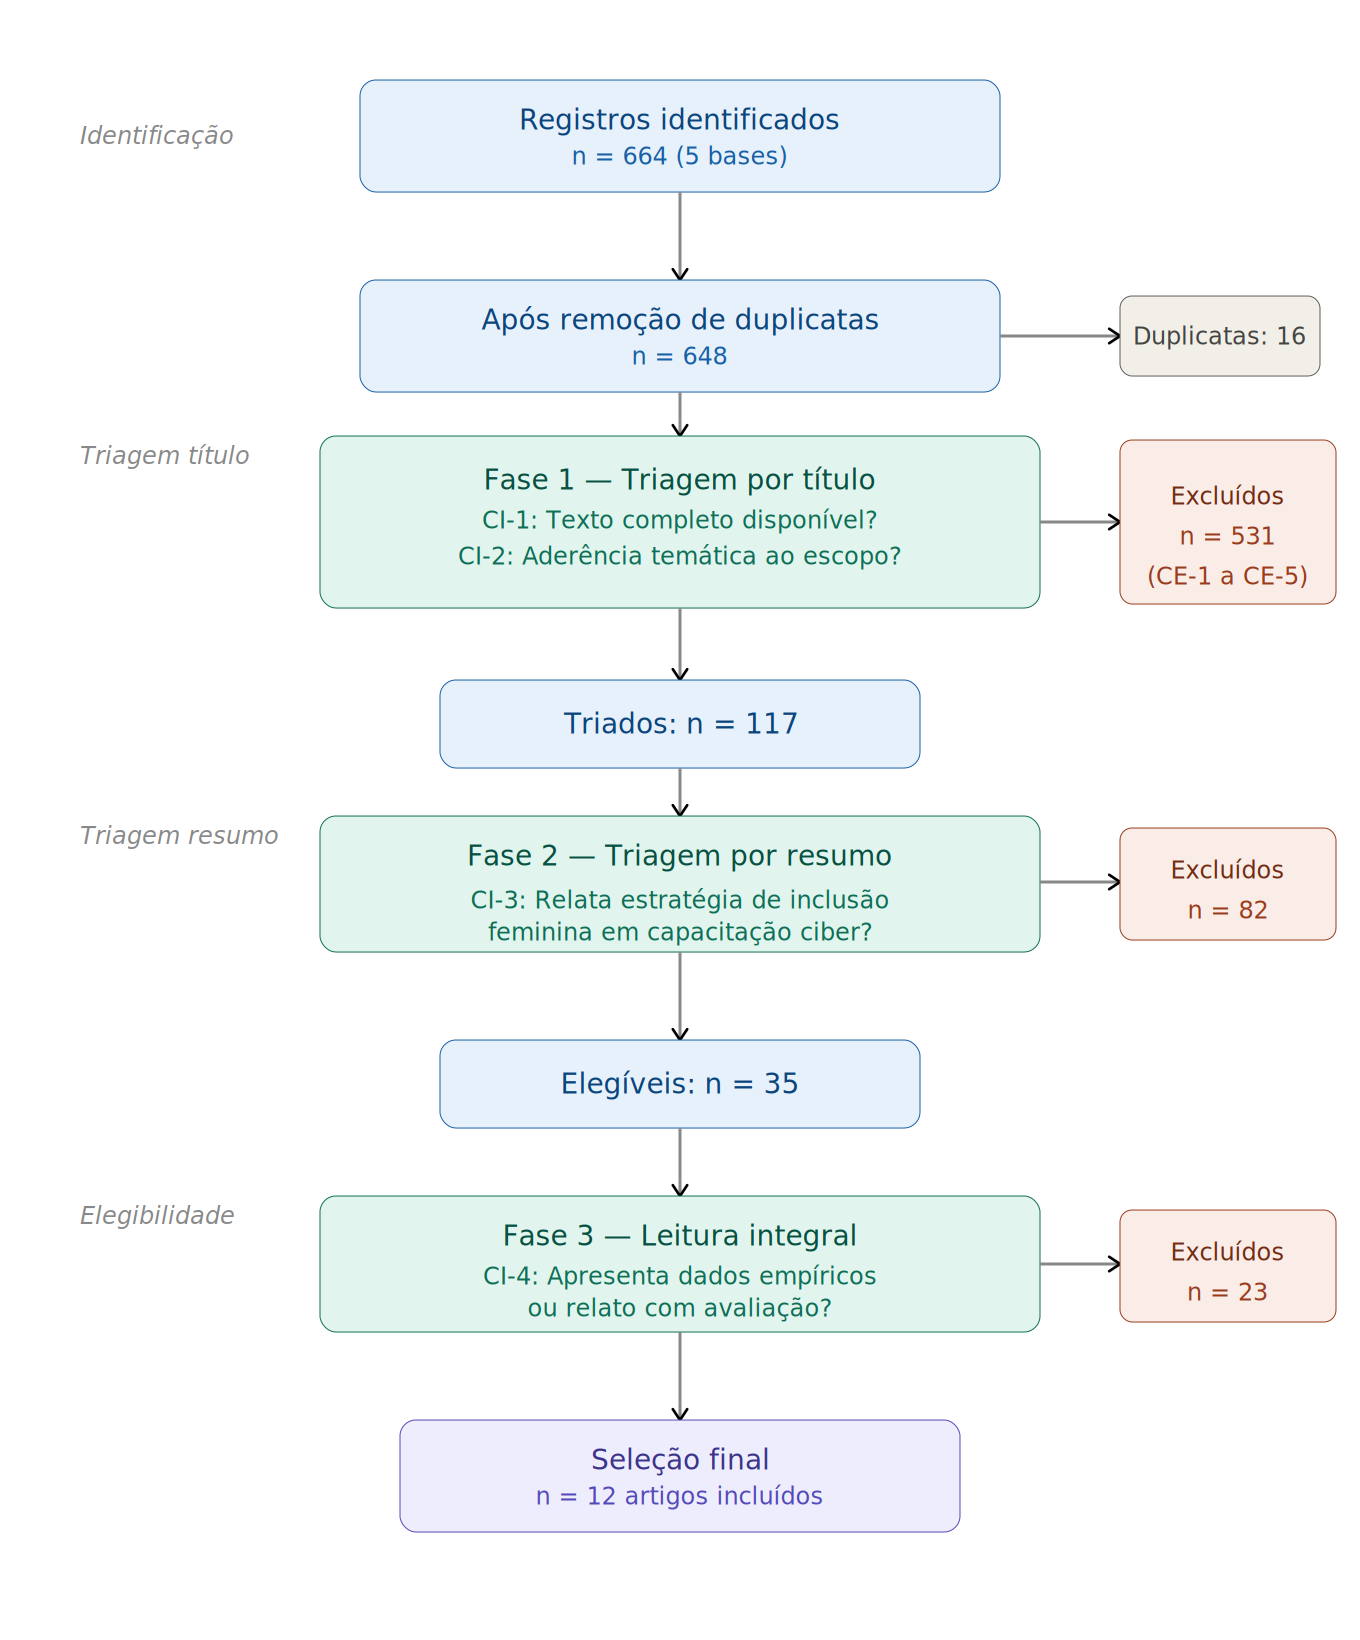
\includegraphics[width=0.7\textwidth]{figs/prisma_flowchart_v2.png}
\caption{Fluxograma PRISMA do processo de seleção}
\label{fig:prisma}
\end{figure}

A Tabela~\ref{tab:selecao} detalha a distribuição dos registros por base de dados ao longo do funil de seleção.

\begin{table}[H]
\centering
\caption{Processo de seleção dos artigos por base de dados}
\label{tab:selecao}
\begin{tabular}{l|c|c|c|c}
\toprule
\textbf{Base de dados} & \textbf{Identificação} & \textbf{Fase~1} & \textbf{Fase~2} & \textbf{Seleção final} \\
\midrule
Google Scholar$^{*}$ & 50  & 29 & 6  & 1 \\
Scopus               & 54  & 23 & 5  & 1 \\
IEEE Xplore          & 342 & 32 & 11 & 1 \\
ACM Digital Library  & 215 & 30 & 10 & 6 \\
SBC Open Lib$^{**}$  & 3  &  3 &  3 & 3 \\
\midrule
\textbf{Total} & \textbf{664}$^{\dagger}$ & \textbf{117} & \textbf{35} & \textbf{12} \\
\bottomrule
\end{tabular}
\vspace{2pt}
\end{table}

A predominância de artigos da ACM Digital Library (50\% da seleção final) reflete a
concentração de publicações sobre educação em computação (\textit{Computing Education})
nessa comunidade científica, com destaque para conferências como SIGCSE TS, ITiCSE e Koli
Calling, além de eventos de segurança como ARES.


% ============================================================
\section{Trabalhos Selecionados} \label{sec:resultados}
% ============================================================

Os 12 artigos selecionados abordam a inclusão de mulheres em cibersegurança sob
perspectivas distintas, organizadas a seguir por temática.

\subsection{Reingresso e Recuperação da Confiança Técnica}

\citeonline{Rahman2022} abordam mulheres em retorno à carreira após afastamento (\textit{career break}), com barreiras de defasagem técnica e baixa autoeficácia (QP1). \textit{Networking} e pares em situação análoga mostram-se tão vitais quanto o conteúdo técnico para retenção (QP3). Limitação: escala reduzida, \textit{workshops} em conferências.

\subsection{Aprendizagem Baseada em Problemas e Andaimes Cognitivos}

\citeonline{Casey2023} apresentam o \textit{Cyber Sleuth Science Lab} (CSSL), baseado em PBL e narrativa investigativa, contextualizando desafios em problemas reais como \textit{cyberbullying} (QP1). Decomposição de tarefas e modelos femininos como facilitadoras aumentaram a autoeficácia (QP2 e QP3). Limitação: mediação síncrona intensa.

\citeonline{Thomas2024} avaliam currículo para comunidades sub-representadas: \textit{scaffolding} (andaimes cognitivos)\footnote{Suportes instrucionais temporários, retirados com o ganho de competência \cite{Wood1976}.} com suportes visuais e extensões de lição mantêm o engajamento (QP2); aulas longas desengajam, sendo necessário intercalar teoria e prática. Limitação: escala reduzida (N=24), \textit{summer camps} presenciais.

\citeonline{SBC_artigo1} relatam oficinas do Projeto \textit{Include Meninas UFF} sobre segurança da informação e \textit{chatbots} (\textit{SecBots}) em escolas públicas. Oficinas desplugadas com conceitos de confidencialidade, integridade e disponibilidade em \textit{design} de diálogo humano-\textit{chatbot} (QP1 e QP2); grupo e facilitadoras reforçam a colaboração (QP3). Três oficinas, 56 participantes (51 meninas). Limitação: escala e aplicação presencial.

\subsection{Gamificação Narrativa e Redução de Ansiedade}

\citeonline{Costa2023} investigam o \textit{CyberTrials} para alunas do ensino médio: \textit{storytelling} com caso de \textit{ransomware} aumenta engajamento e autoeficácia (QP2); a ``camada de apresentação'' do conteúdo é tão importante quanto o técnico.

\citeonline{Costa2025} validam o mesmo programa com RPG e pré/pós-testes (779 alunas). Narrativa ``detetives'' em vez de ``hackers'' reduziu estereótipo e aumentou intenção de carreira em STEM (QP1 e QP2); colaboração no RPG foi determinante para o engajamento (QP3).

\subsection{Mentoria, Empregabilidade e \textit{Soft Skills}}

\citeonline{Musuva2025} documentam o \textit{Cyber Shujaa} (Quênia): capacitação prática, imersão em empresas e colocação no mercado; 41\% de participação feminina via recrutamento afirmativo (QP1). Mentoria fortalece identidade e mitiga síndrome do impostor (QP3). Limitação: baixa escalabilidade do modelo presencial.

\citeonline{Benson2025} investigam, pela Teoria Social Cognitiva de Carreira, \textit{soft skills} (resiliência, comunicação, liderança) como proteção ao isolamento feminino (QP1). Quatro pilares: confiança, mentoria, colaboração e políticas inclusivas; aprendizado colaborativo combate síndrome do impostor (QP3). Carece de proposta para EAD.

\citeonline{SBC_artigo3} documentam o \textit{Ladies in Cyber} (Itaipu Parquetec): treinamentos, palestras, eventos, mentoria e parcerias para estágios e empregos; trilha inaugural com 32 vagas (QP1--QP3). Representatividade e ambientes acolhedores reduzem barreiras. Limitação: centro específico, escala local.

\citeonline{SBC_artigo2} mapeiam ações e iniciativas para inclusão de mulheres em cibersegurança no Brasil (Scopus, \textit{Web of Science}, Google Acadêmico, SBSeg, WIT), identificam carência no país (um artigo e cinco projetos) e propõem ações a partir de iniciativas internacionais (QP1). Estudo secundário; mantido por mapear iniciativas brasileiras e propor ações alinhadas às QPs.

\subsection{Escalabilidade e Plataformas Abertas}

\citeonline{Tshekiso2025} documentam a \textit{picoCTF-Africa}: plataformas abertas e \textit{hardware} agnóstico escalam o ensino em múltiplos países africanos (QP2); clubes locais e categoria para mulheres (QP1) mostram que competição aberta sozinha não garante equidade. Limitação: sem pedagogia de gênero além da categoria.

\citeonline{Hogan2025} investigam \textit{swift trust} em equipes distribuídas em CTF remotas: autoeficácia amplia-se quando o ambiente virtual simula um laboratório físico; plataformas massivas devem incorporar comunidades persistentes (QP3). Limitação: foco em times de sucesso, viés de sobrevivência.


% ============================================================
\section{Análise e Discussão} \label{sec:analise}
% ============================================================

\subsection{Distribuição Temporal}

A análise temporal revela concentração em 2023 (três artigos) e 2025 (sete), com um trabalho em 2022 e um em 2024, indicando tema emergente e de alta relevância.

\subsection{Análise Multidimensional}

Os trabalhos foram avaliados em cinco dimensões (QP1--QP3, Escalabilidade, Avaliação Empírica). A Tabela~\ref{tab:comparacao} sintetiza a comparação qualitativa.

\begin{table}[H]
\centering
\caption{Comparação dos trabalhos selecionados por dimensão de análise}
\label{tab:comparacao}
\begin{tabular}{l|c|c|c|c|l}
\toprule
\textbf{Trabalho} & \textbf{Gênero} & \textbf{Ped.} & \textbf{Colab.} & \textbf{Escala} & \textbf{\textit{Gap} principal} \\
\midrule
Costa et al.    & Alta  & Alta  & Méd. & Méd. & Sem dados longitudinais de carreira \\
Musuva et al.  & Méd.  & Méd.  & Alta & Méd. & Modelo presencial, difícil de escalar \\
Tshekiso et al. & Bx. & Bx.  & Méd. & Alta & Sem pedagogia específica de gênero \\
Benson et al.  & Alta  & Bx.   & Alta & Bx.  & Sem plataforma EAD aplicada \\
Costa et al.    & Alta  & Alta  & Alta & Méd. & Foco em atração, não em retenção \\
Casey et al.    & Alta  & Alta  & Alta & Bx.  & Dependência de mediação síncrona \\
Thomas et al.  & Alta  & Alta  & Bx.  & Bx.  & Amostra pequena (N=24) \\
Rahman et al.  & Alta  & Méd.  & Alta & Bx.  & Foco em reingresso, escala reduzida \\
Hogan et al.    & Bx.   & Méd.  & Alta & Alta & Viés de sobrevivência, times mistos \\
Salgado et al. & Alta  & Alta  & Alta & Bx.  & Oficina desplugada, escala reduzida \\
Holanda et al. & Méd.  & Bx.   & Bx.  & Bx.  & Mapeamento, sem intervenção empírica \\
Pereira et al. & Alta  & Méd.  & Alta & Méd. & Iniciativa local, 32 vagas na trilha \\
\bottomrule
\end{tabular}
\end{table}

\subsubsection{Foco em Gênero e Barreiras (QP1)}

Oito dos 12 artigos têm alto foco em gênero. Barreiras: (i) \textbf{estruturais}, ausência de \textit{role models} e currículos com viés; (ii) \textbf{culturais}, estereótipos de domínio masculino; (iii) \textbf{pedagógicas}, gamificação competitiva que eleva ansiedade de \textit{performance}. Destacam-se \cite{Costa2025} e \cite{Benson2025} no combate a estereótipos e no fortalecimento da identidade profissional feminina.

\subsubsection{Abordagens Pedagógicas (QP2)}

Os trabalhos de maior foco pedagógico \cite{Costa2023, Costa2025, Casey2023, Thomas2024} convergem em: (i) contextualização narrativa em problemas sociais reais; (ii) andaimes cognitivos para reduzir carga cognitiva; (iii) colaboração em vez de competição individual. A eficácia inclusiva depende de transformar a cibersegurança de arena competitiva em espaço de investigação e impacto social.

\subsubsection{Colaboração e Autoeficácia (QP3)}

Mecanismos eficazes: \textbf{comunidades de prática} \cite{Hogan2025, Tshekiso2025}, \textbf{mentoria formal} \cite{Musuva2025} e \textbf{\textit{soft skills}} \cite{Benson2025}. A autoeficácia pode ser fortalecida por intervenções que valorizem identidade profissional e colaboração.

\subsubsection{Escalabilidade e Avaliação Empírica}

\cite{Tshekiso2025} e \cite{Hogan2025} operam em plataformas digitais escaláveis, mas sem adaptações de gênero; as intervenções pedagogicamente mais eficazes \cite{Casey2023, Thomas2024} são presenciais e pouco escaláveis. \cite{Costa2025} e \cite{Casey2023} destacam-se em rigor metodológico (grupos de controle, dados longitudinais).

\subsection{Lacunas Identificadas}

A análise revela uma dicotomia: intervenções inclusivas de pequena escala vs. modelos escaláveis sem recorte de gênero. A \textbf{lacuna principal} é a ausência de um modelo que operacionalize mentoria e \textit{soft skills} em ambientes assíncronos de alcance nacional, embora \cite{Musuva2025} e \cite{Benson2025} evidenciem a eficácia dessas práticas em escala reduzida.


% ============================================================
\section{Considerações Finais} \label{sec:conclusao}
% ============================================================

Este artigo apresentou os resultados de uma RSL sobre programas de capacitação de
mulheres em cibersegurança, conduzida em cinco bases de dados. A partir de 664 registros identificados, 12 artigos foram selecionados, representando o estado da arte sobre o tema.

Os principais achados indicam que: (1) as barreiras à participação feminina são
multidimensionais, combinando fatores estruturais, culturais e pedagógicos; (2) a
\textbf{gamificação narrativa} e o \textbf{\textit{scaffolding} cognitivo} são as
abordagens pedagógicas mais eficazes para o público feminino iniciante; (3)
\textbf{mentoria formal} e \textbf{comunidades de prática} são mecanismos indispensáveis
de retenção; e (4) existe uma lacuna crítica entre intervenções inclusivas de pequena
escala e programas massivos, que precisa ser preenchida por modelos que integrem ambas
as dimensões simultaneamente.

A revisão evidencia a necessidade de pesquisas situadas no contexto brasileiro. Os resultados desta RSL fundamentam a construção de um \textit{Framework} de Diretrizes para Inclusão e Retenção de Mulheres em Programas de Capacitação em Cibersegurança, cujo desenvolvimento constitui o objetivo central da dissertação de mestrado da qual este artigo é derivado.

Como trabalho futuro, pretende-se: (i) validar o \textit{framework} proposto junto a um
painel de especialistas em cibersegurança, educação e diversidade; e (ii) avaliar a
percepção de utilidade com alunas do Programa \textit{Hackers} do Bem, ativas e evadidas,
por meio de \textit{survey} fundamentado no Modelo ARCS (Atenção, Relevância, Confiança e Satisfação) de motivação instrucional \cite{Keller1987}.

\subsection*{Uso de Inteligência Artificial}

Não foi utilizada inteligência artificial generativa na elaboração deste artigo.

\bibliographystyle{styles/abntex2-alf}
\bibliography{bibliography/references}

\end{document}
